% Ergebnisse - Endergebnisse der Arbeit, Performance, Bilder (auf dpi achten, mind. 300), Kennkurven, Warps, weitere Leistungsmessungen bez. auf meine Arbeit
% -> ggf. Results and Discussion seperat halten
% Bedeutung der Ergebnisse (im Rahmen dessen was wissenschaftlich haltbar ist)
\chapter{Ergebnisse und Diskussion}\label{chap::resdisc}
Dieses Kapitel beinhaltet die Ergebnisse dieser Arbeit und eine anschließende Diskussion der Messwerte und der Umsetzung verschiedener Arbeitspakete.
Der erste Abschnitt behandelt dabei die Bildqualität der Ergebnisse.
Der zweite Abschnitt beinhaltet Messungen zur Performanz der verschiedenen Raycast Implementierungen bezüglich der Ausführungszeiten sowie der Nutzbarkeit in Verbindung mit einem Eye Tracker.
Im zweiten Abschnitt werden diese näher diskutiert.

\section{Ergebnisse}\label{sec::results}
Der erste Abschnitt beinhaltet Ergebnissen der Implementierungen \emph{MDC} \ref{ss::MDC} und \emph{DDC} \ref{ss::DDC} sowie der ursprünglichen Implementierung des Raycasts \ref{ss::rc} aus Sicht der Bildqualität.
Der zweite Abschnitt beinhaltet gemessene Performanzleistungen der jeweiligen Implementierungen bei der Verwendung unterschiedlicher Transferfunktionen und Volumendaten.

\subsection{Bildqualität}
Im folgenden werden zu den Implementierungen \emph{MDC}, \emph{DDC} und als Vergleich zur Ursprünglichen Implementierung Screenshots gezeigt, welche die Bildqualität der Implementierungen darstellen sollen.
Dies wird anhand von zwei verschiedenen Volumen mit jeweils einer Transferfunktion dargestellt.
Für jedes der Volumen wird jeweils das Bild in normaler Auflösung, welche mit der ursprünglichen Implementierung berechnet wurde sowie das Ergebnis der Berechnung des Bildes durch \emph{MDC} und \emph{DDC} gezeigt.
Bei den Berechnungen durch \emph{MDC} und \emph{DDC} werden die jeweils verwendeten Parameter der Berechnung angegeben.

\subsubsection{Standard Raycast}\label{ss::res::sr}
Abbildung \ref{fig::res::bon_st} zeigt eine Berechnung des Volumens \emph{Bonsai} mit dem ursprünglichen Raycast.
Die ursprüngliche Implementierung berechnete das gesamte Bild mit normaler Auflösung.
Das heißt, dass für jeden Pixel des Bildes ein Work-Item gestartet wurde, um den Raycast eines Strahls zu berechnen.
Der jeweilige Pixel erhält die berechnete Farbe des Work-Items.
Die Abtastrate der Strahlen hat den Standardwert von $1.5$\,Tastungen pro Voxel.
Durch die Interpolation der Voxel wird das Volumen mit weichen Konturen und Flächen gezeichnet.
Die Transferfunktion hebt die Voxel mit etwas höherer Dichte farblich hervor.
Dies entspricht hier dem Stamm und den Ästen sowie der Erde und der Schale, in welcher sich der Bonsai befindet.
Die Blätter werden teilweise ausgeblendet.
Die Grashalme, die aus der Erde sprießen, sind vollständig ausgeblendet.
Insgesamt sind werden die Flächen aber transparent gezeichnet, so dass auch eigentlich verdeckte Strukturen zu sehen sind.

\begin{landscape}
	\begin{figure}
		\centering
		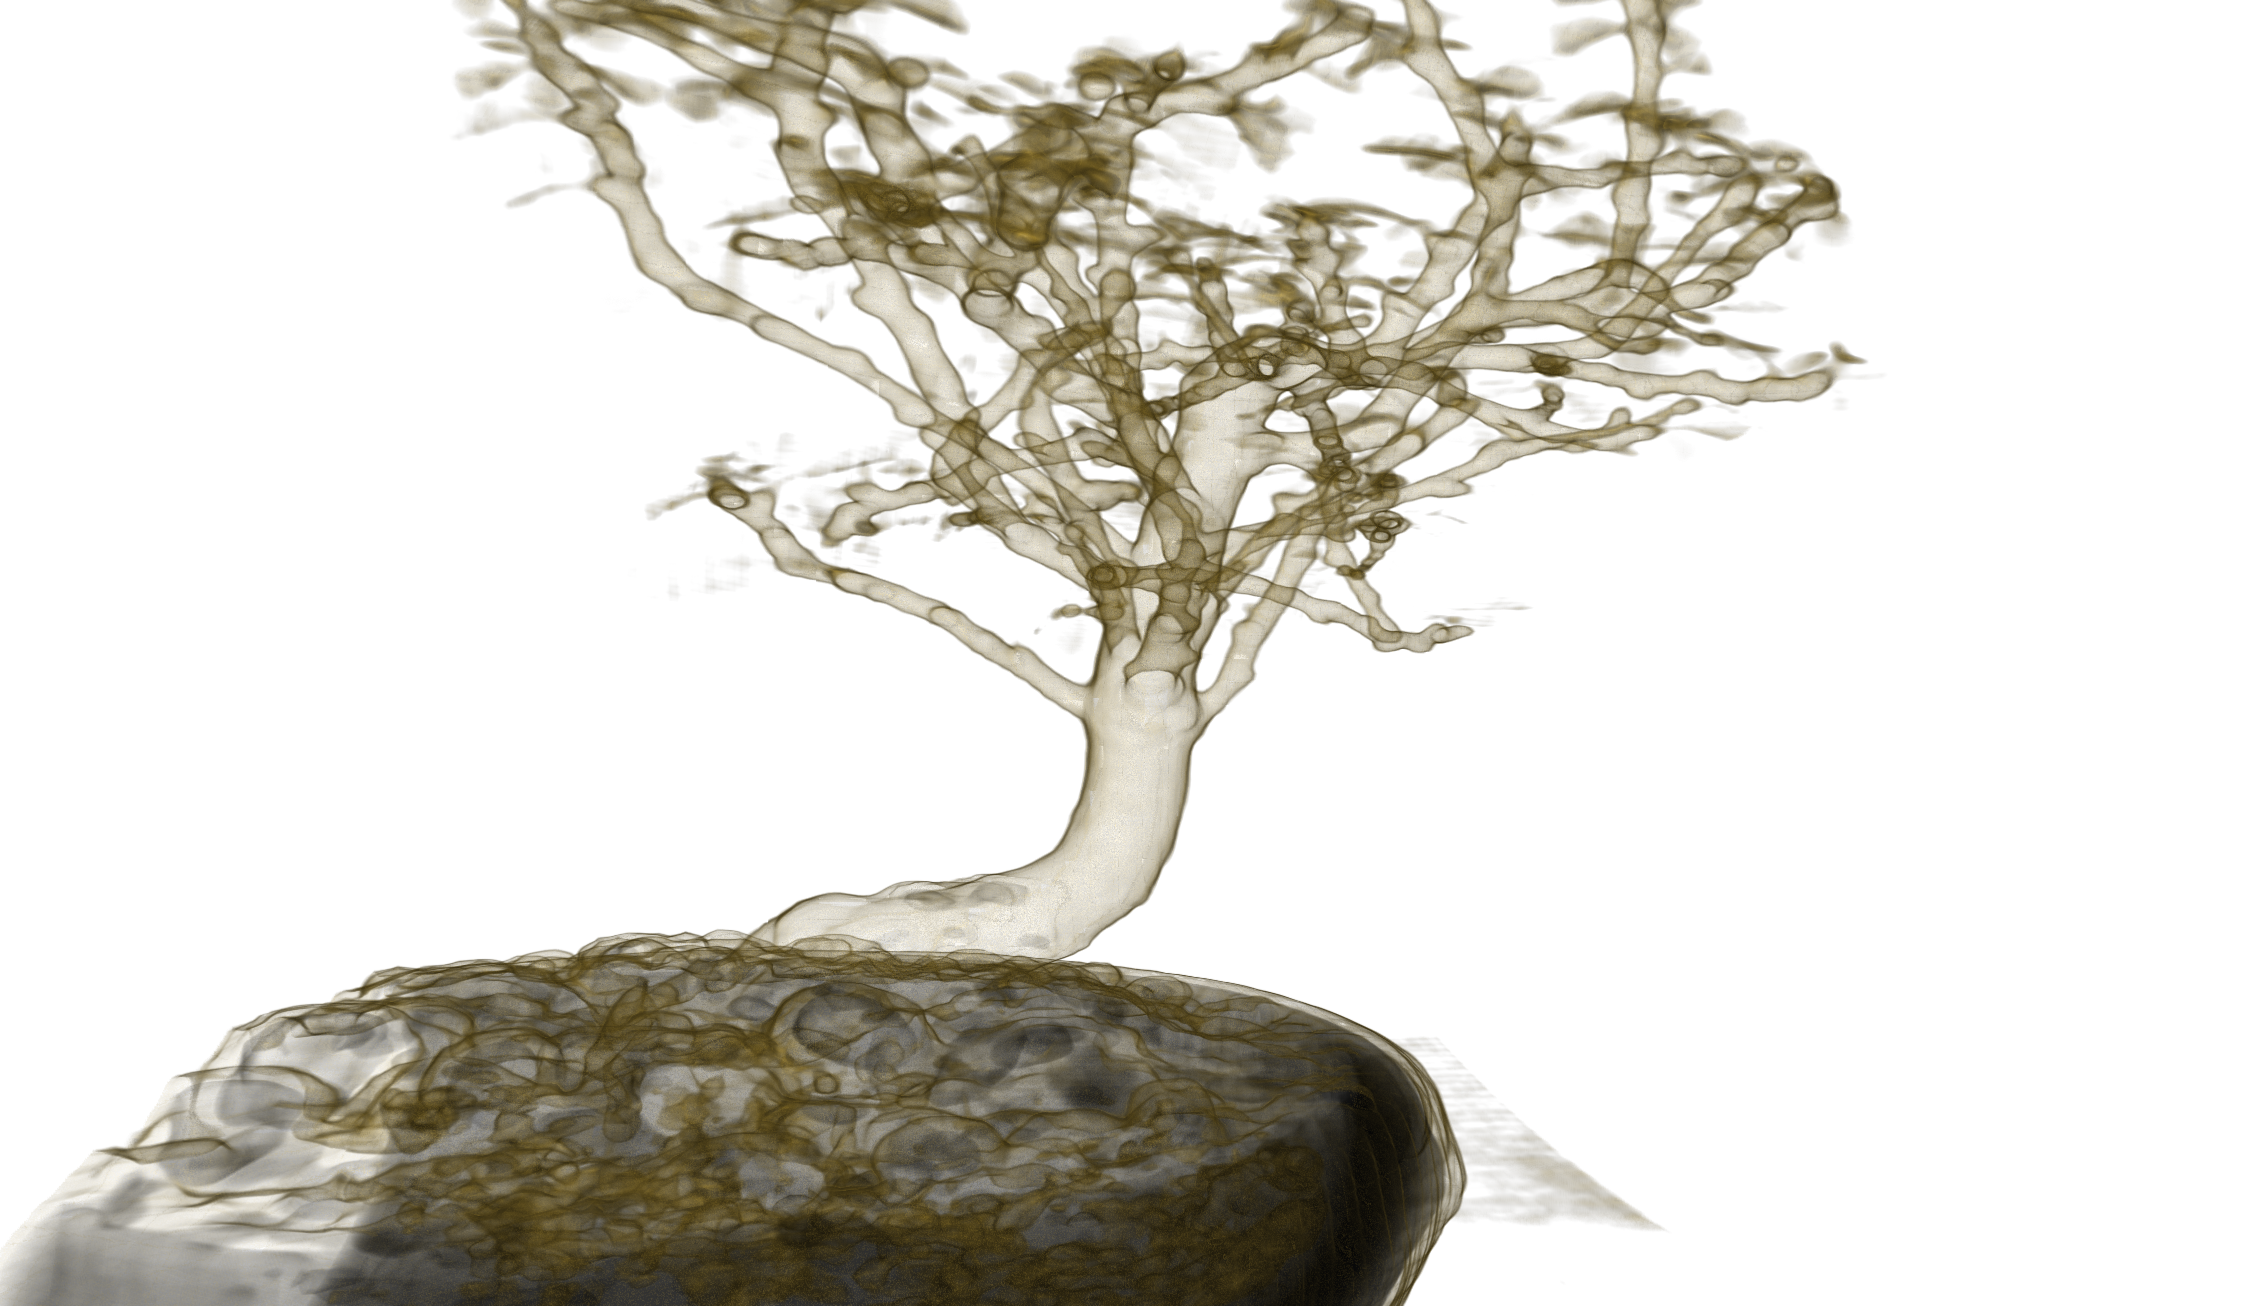
\includegraphics[width=\textheight]{../../Grafiken/results/picture_quality/bonsai/Standard_img-1_Ray-1-5.png}
		\caption{Volumen Bonsai mit ursprünglichem Raycast berechnet.}
		\label{fig::res::bon_st}
	\end{figure}
\end{landscape}

\subsubsection{MDC Raycast}\label{ss::res::mdc}
Der \emph{MDC} Raycast ist das Ergebnis des Arbeitspakets, aus dem Abschnitt \ref{ss::MDC}.
Die Abbildung \ref{fig::res::bon_mdc} zeigt das Volumen \emph{Bonsai}, welches mit dem \emph{MDC} Raycas berechnet wurden.
Das Bild wurde dabei aus der selben Perspektive und mit der gleichen Transferfunktion berechnet, wie dies auch in Abbildung \ref{fig::res::bon_st} der Fall war.
Die Strahlabtastrate ist ebenfalls gleich wie bei der Berechnung des Bildes in Abbildung \ref{fig::res::bon_st}, welches mit dem Standard Raycast berechnet wurde.
Die Bildabtastrate hat statt einem Wert von $1$ einen Wert von $0.96$.
Damit wird einer leichten Verschiebung des Bildes, aufgrund der zwei unterschiedlichen Auflösungen, entgegengewirkt.

In diesem Fall, beim \emph{MDC} Raycast, wurde zwei Bilder berechnet, welche anschließend passend zusammengefügt wurden.
Das erste Bild wurde mit nur einem viertel der Auflösung berechnet und anschließend auf die normale Auflösung interpoliert.
Das zweite Bild wurde mit der normalen Auflösung berechnet, dafür aber nur ein rechteckiger Ausschnitt an der Mausposition.
Das zweite Bild wurde anschließend an der Mausposition in das auf die normale Auflösung interpolierte erste Bild eingefügt.

\todo{Mausposition in das Bild einzeichnen.}
An den Konturen der Abbildung \ref{fig::res::bon_mdc} ist ein leichter Abfall der Auflösung des Bildes zu erkennen.
Die Konturen, welche in Abbildung \ref{fig::res::bon_st} noch weich gezeichnet wurden, haben außerhalb des Rechtecks um die Mausposition nun Artefakte der Unterabtastung, wie zum Beispiel leichte Treppenstufen.
Innerhalb des Rechtecks sind die Konturen immer noch weich gezeichnet und es ist dort kein Unterschied zu Abbildung \ref{fig::res::bon_st} zu sehen.

\begin{landscape}
	\begin{figure}
		\centering
		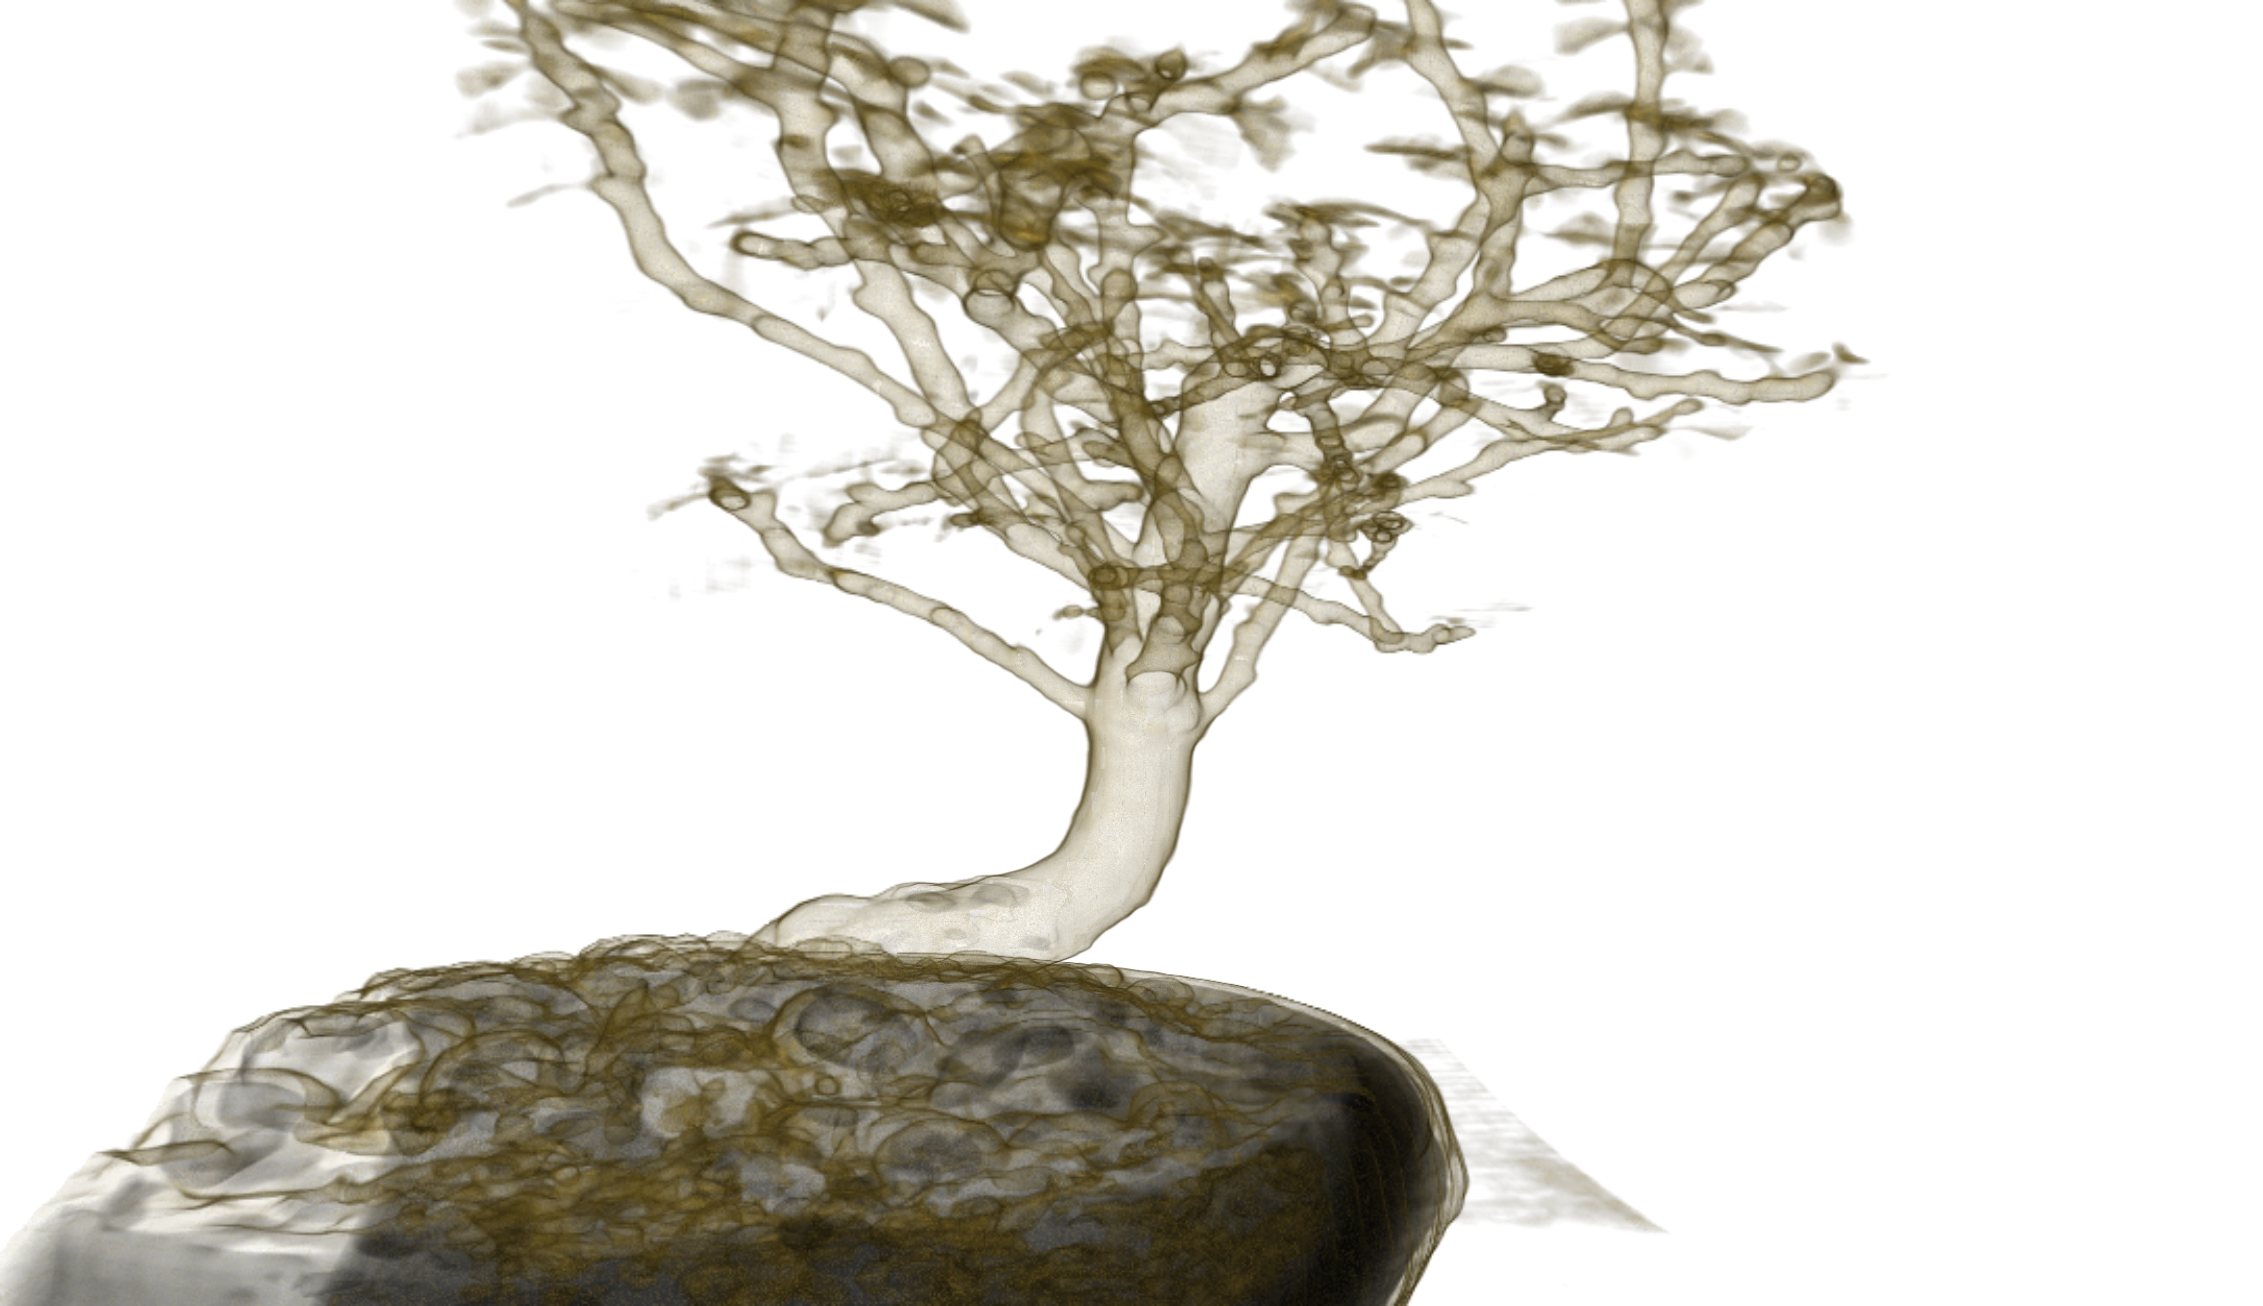
\includegraphics[width=1\textheight]{../../Grafiken/results/picture_quality/bonsai/MDC_img-0-96_ray-1-5.png}
		\caption{Volumen Bonsai mit \emph{MDC} Raycast berechnet.}
		\label{fig::res::bon_mdc}
	\end{figure}
\end{landscape}

\subsubsection{DDC Raycast}\label{ss::res::ddc}
Der \emph{DDC} Raycast ist das Ergebnis, des Arbeitspakets aus dem Abschnitt

\begin{landscape}
	\begin{figure}
		\centering
		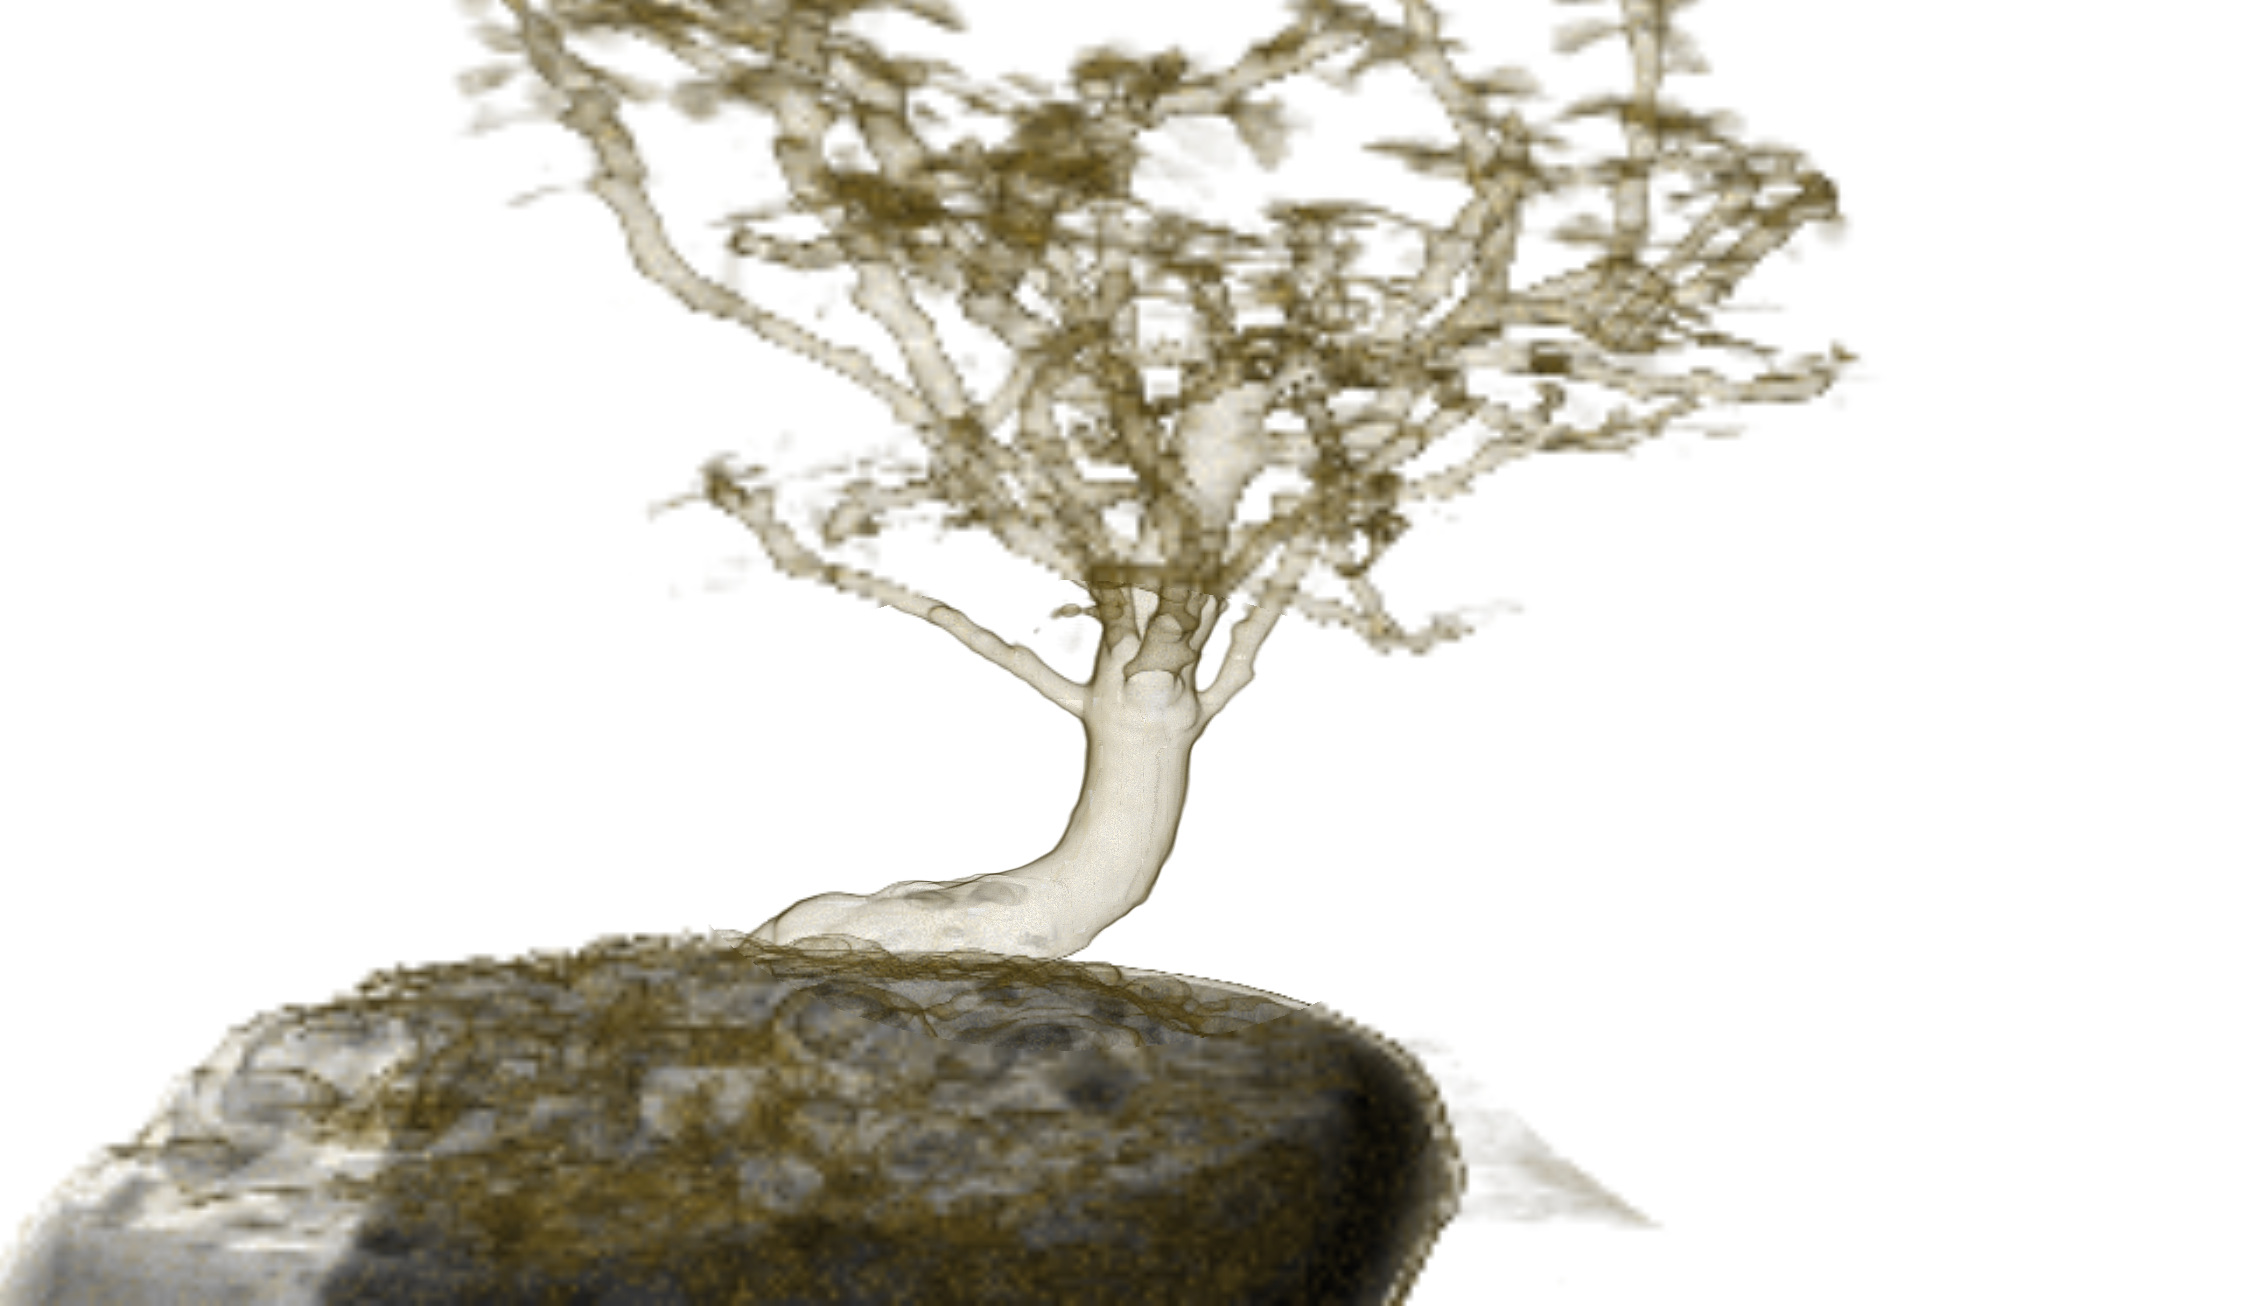
\includegraphics[width=1\textheight]{../../Grafiken/results/picture_quality/bonsai/DDC_img-1_ray-1-5.png}
		\caption{Volumen Bonsai mit \emph{DDC} Raycast berechnet.}
		\label{fig::res::bon_ddc}
	\end{figure}
\end{landscape}

\iffalse




\begin{landscape}
	\begin{figure}
		\centering
		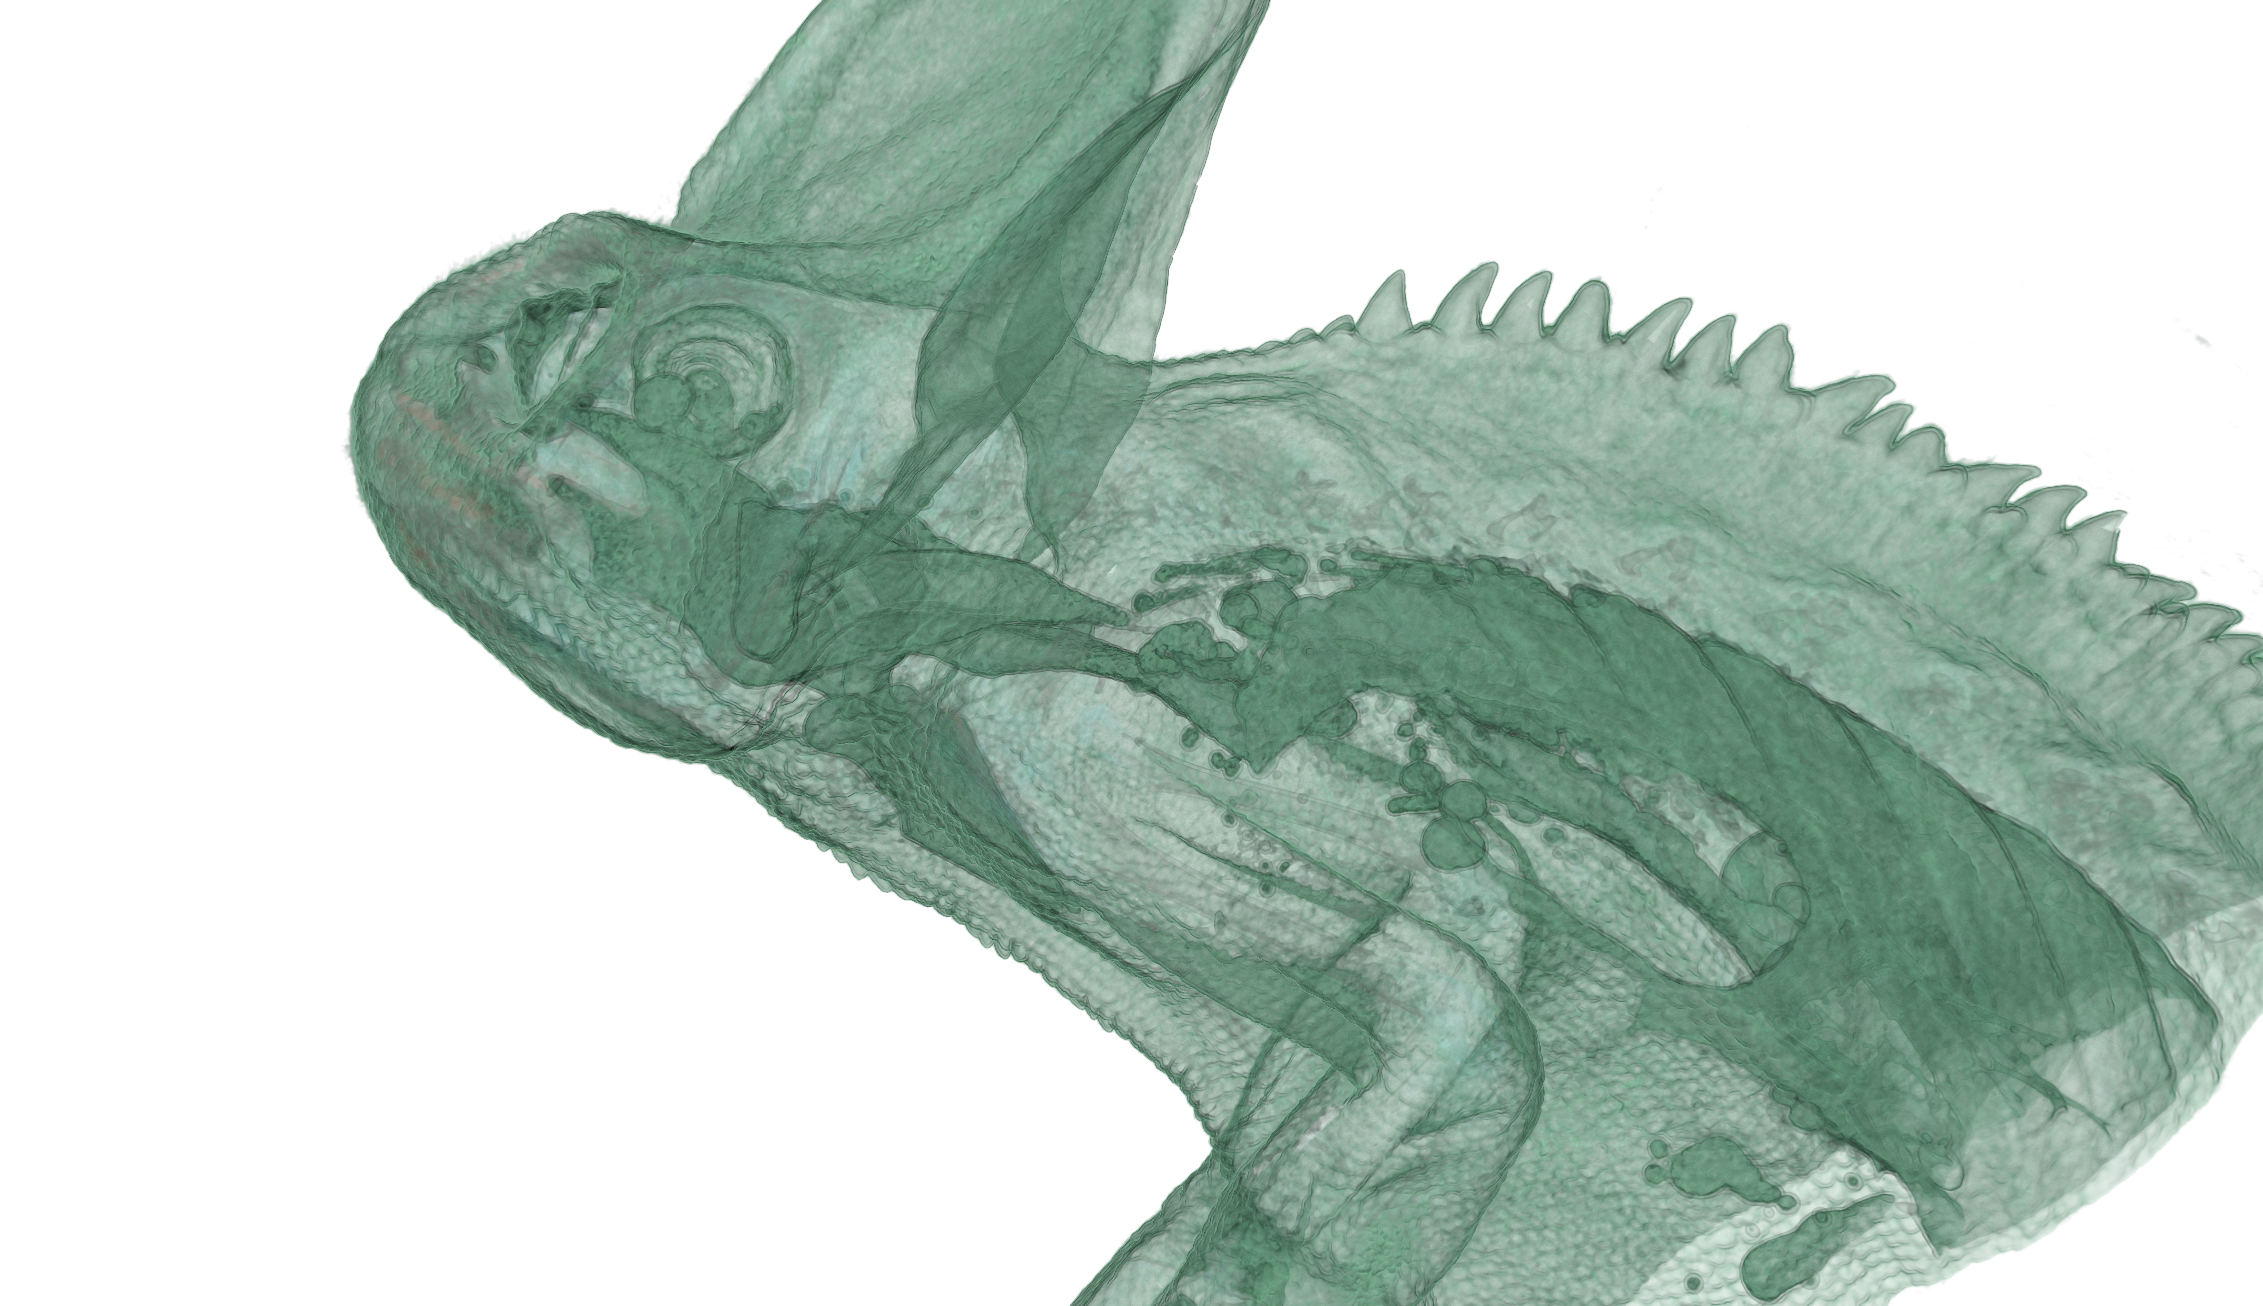
\includegraphics[width=1\textheight]{../../Grafiken/results/picture_quality/chameleon/Standard_img-1_Ray-1-5.png}
		\caption{Volumen Chameleon mit ursprünglichem Raycast berechnet.}
		\label{fig::res::cam_st}
	\end{figure}
\end{landscape}

\begin{landscape}
	\begin{figure}
		\centering
		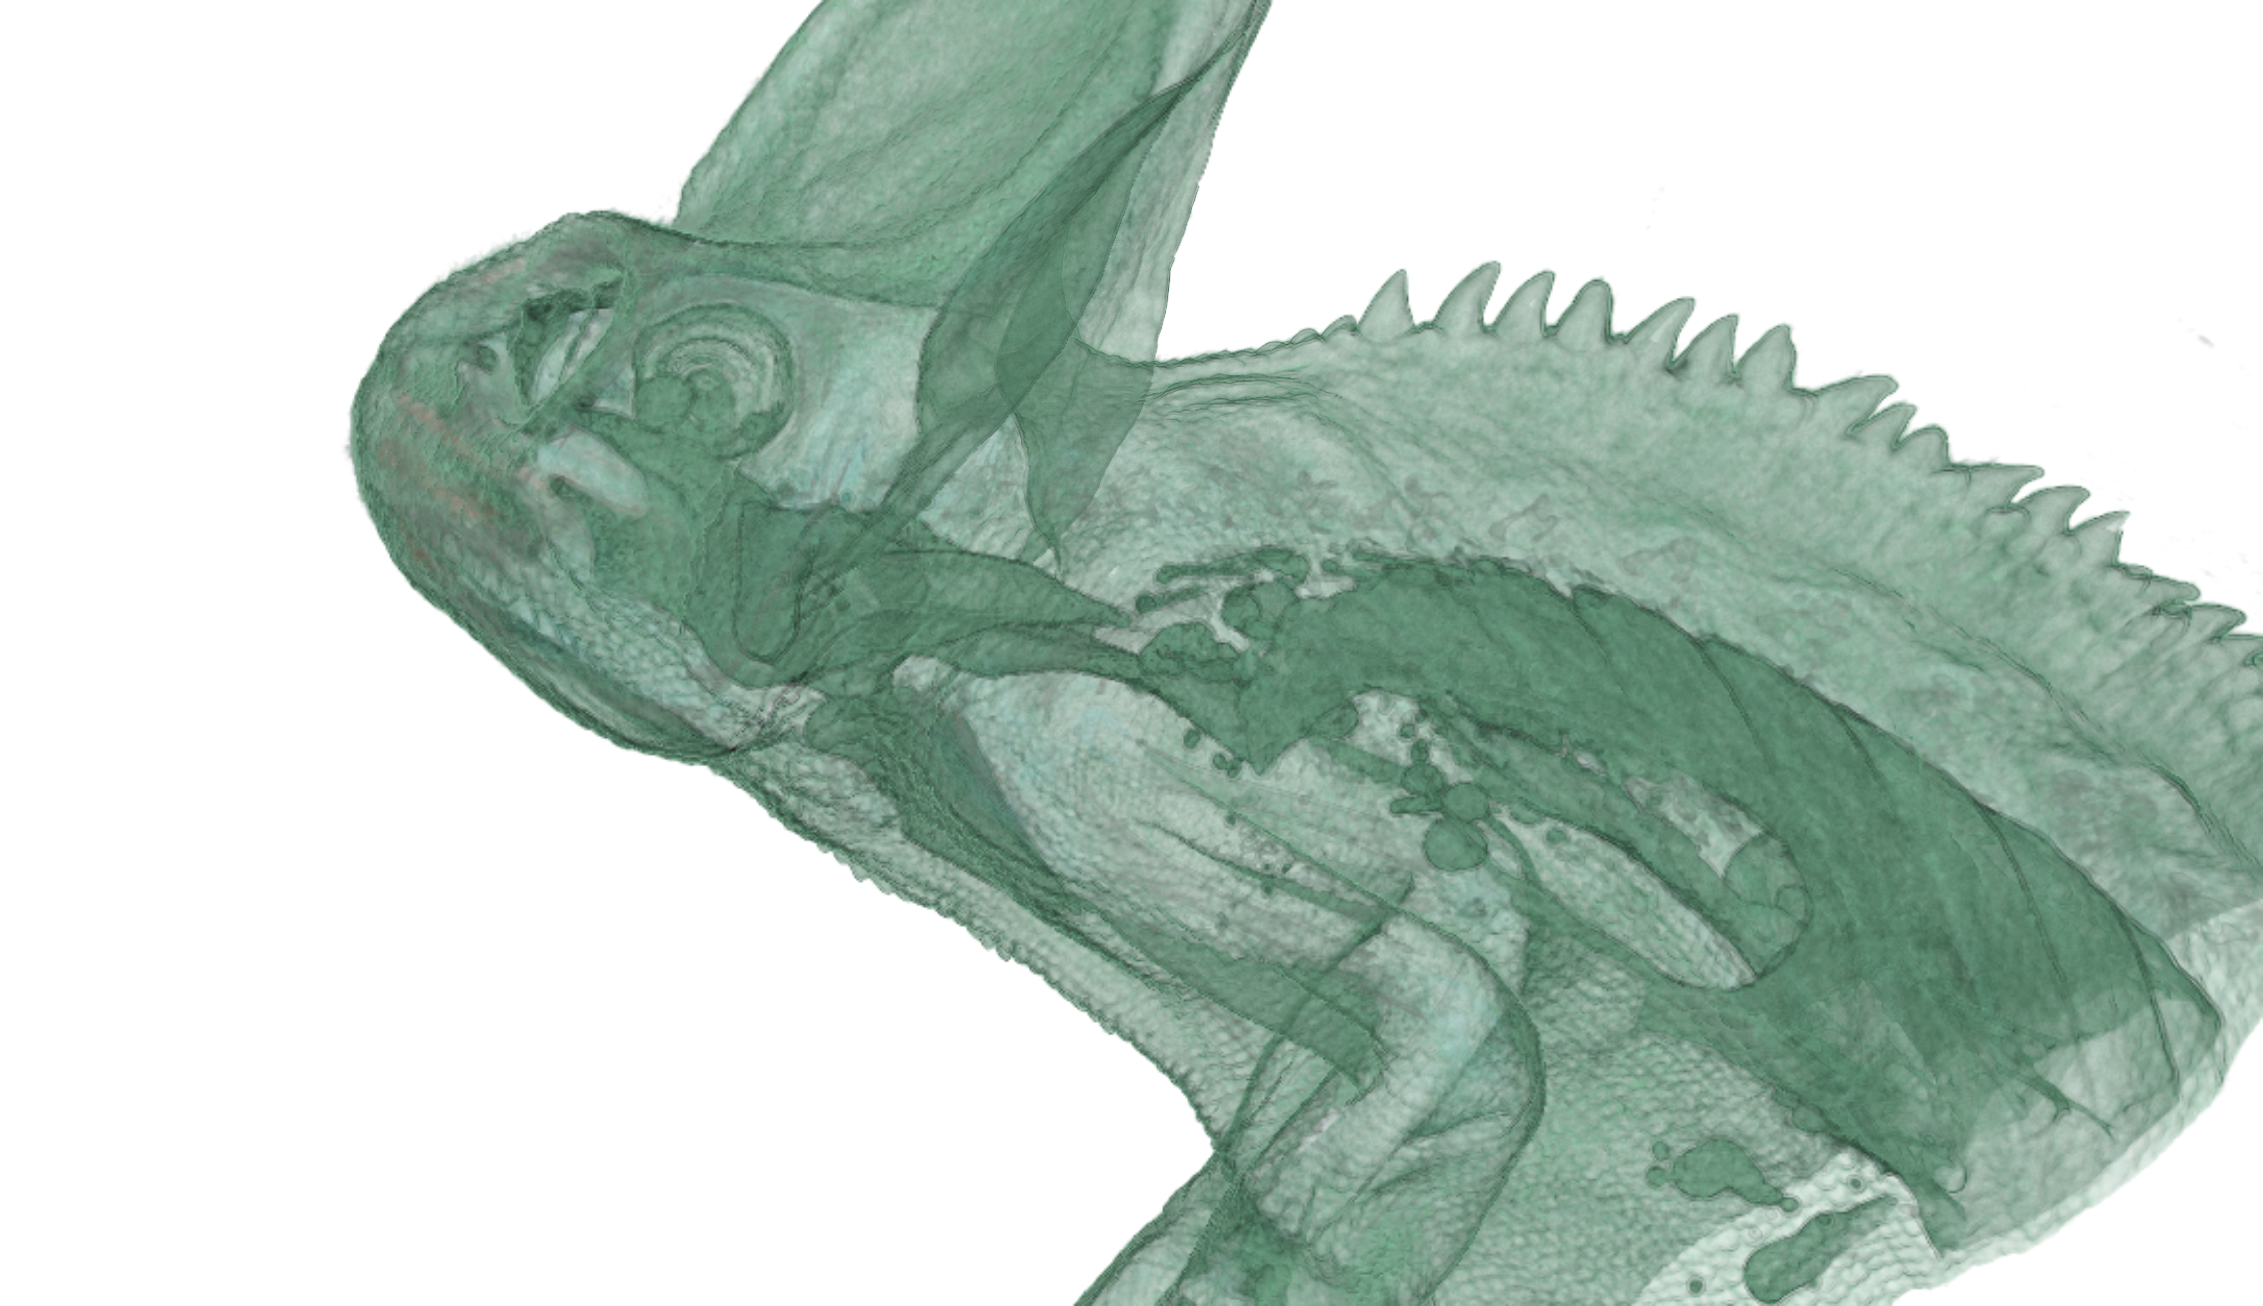
\includegraphics[width=1\textheight]{../../Grafiken/results/picture_quality/chameleon/MDC_img-0-96_ray-1-5.png}
		\caption{Volumen Chameleon mit \emph{MDC} Raycast berechnet.}
		\label{fig::res::cam_mdc}
	\end{figure}
\end{landscape}

\begin{landscape}
	\begin{figure}
		\centering
		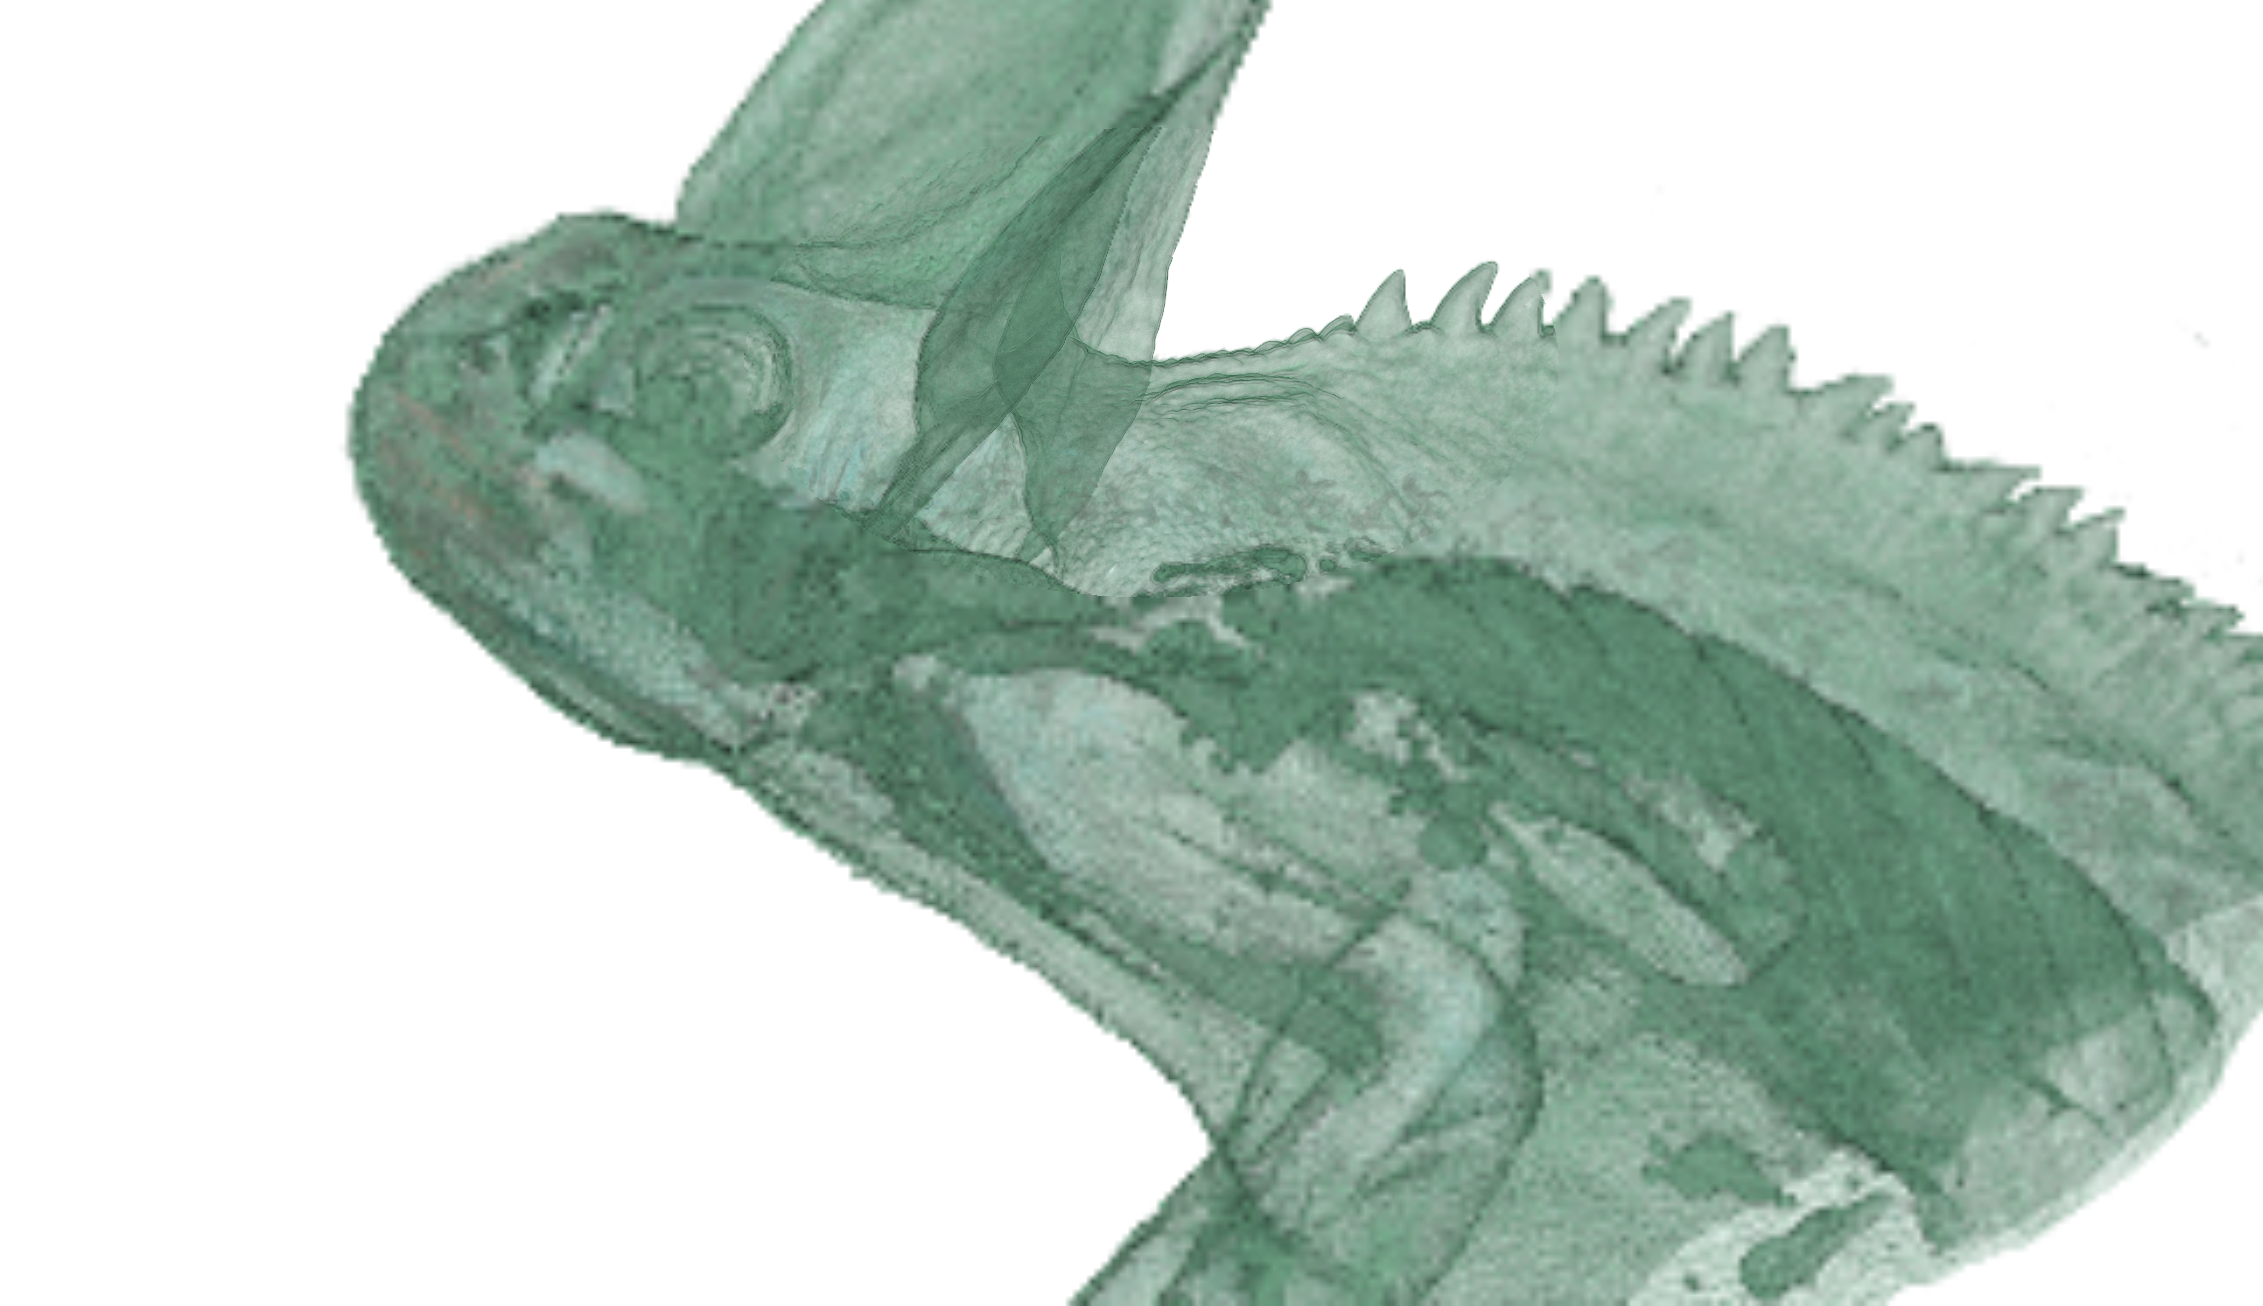
\includegraphics[width=1\textheight]{../../Grafiken/results/picture_quality/chameleon/DDC_img-1_ray-1-5.png}
		\caption{Volumen Chameleon mit \emph{DDC} Raycast berechnet.}
		\label{fig::res::cam_ddc}
	\end{figure}
\end{landscape}


\begin{landscape}
	\begin{figure}
		\centering
		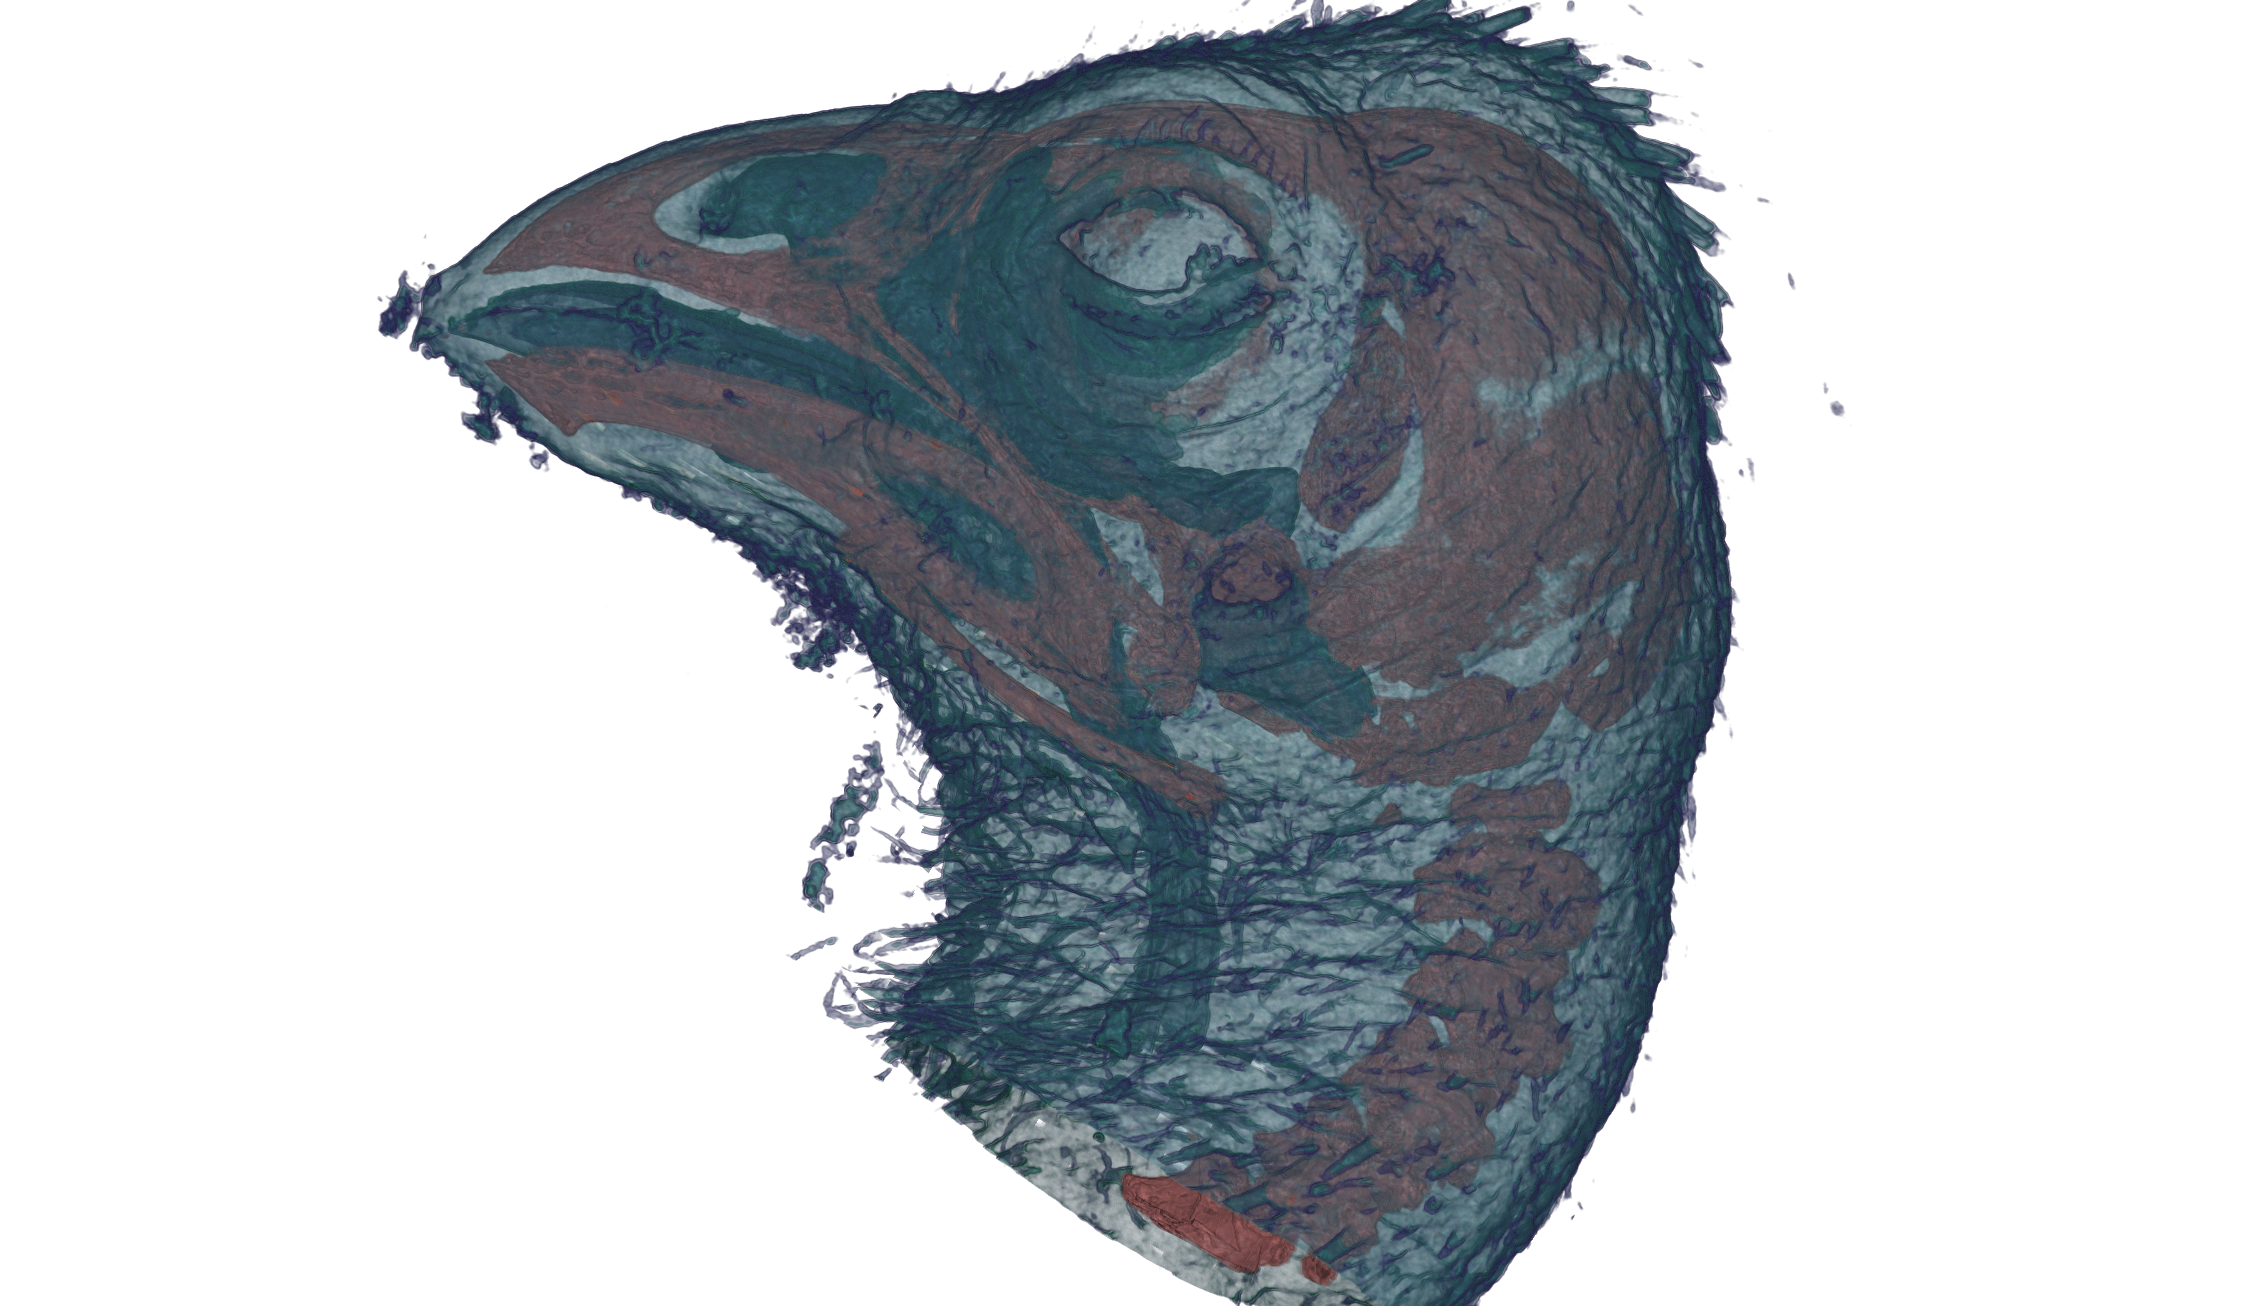
\includegraphics[width=1\textheight]{../../Grafiken/results/picture_quality/hoatzin/Standard_img-1_Ray-1-5.png}
		\caption{Volumen Hoatzin mit ursprünglichem Raycast berechnet.}
		\label{fig::res::hoa_st}
	\end{figure}
\end{landscape}

\begin{landscape}
	\begin{figure}
		\centering
		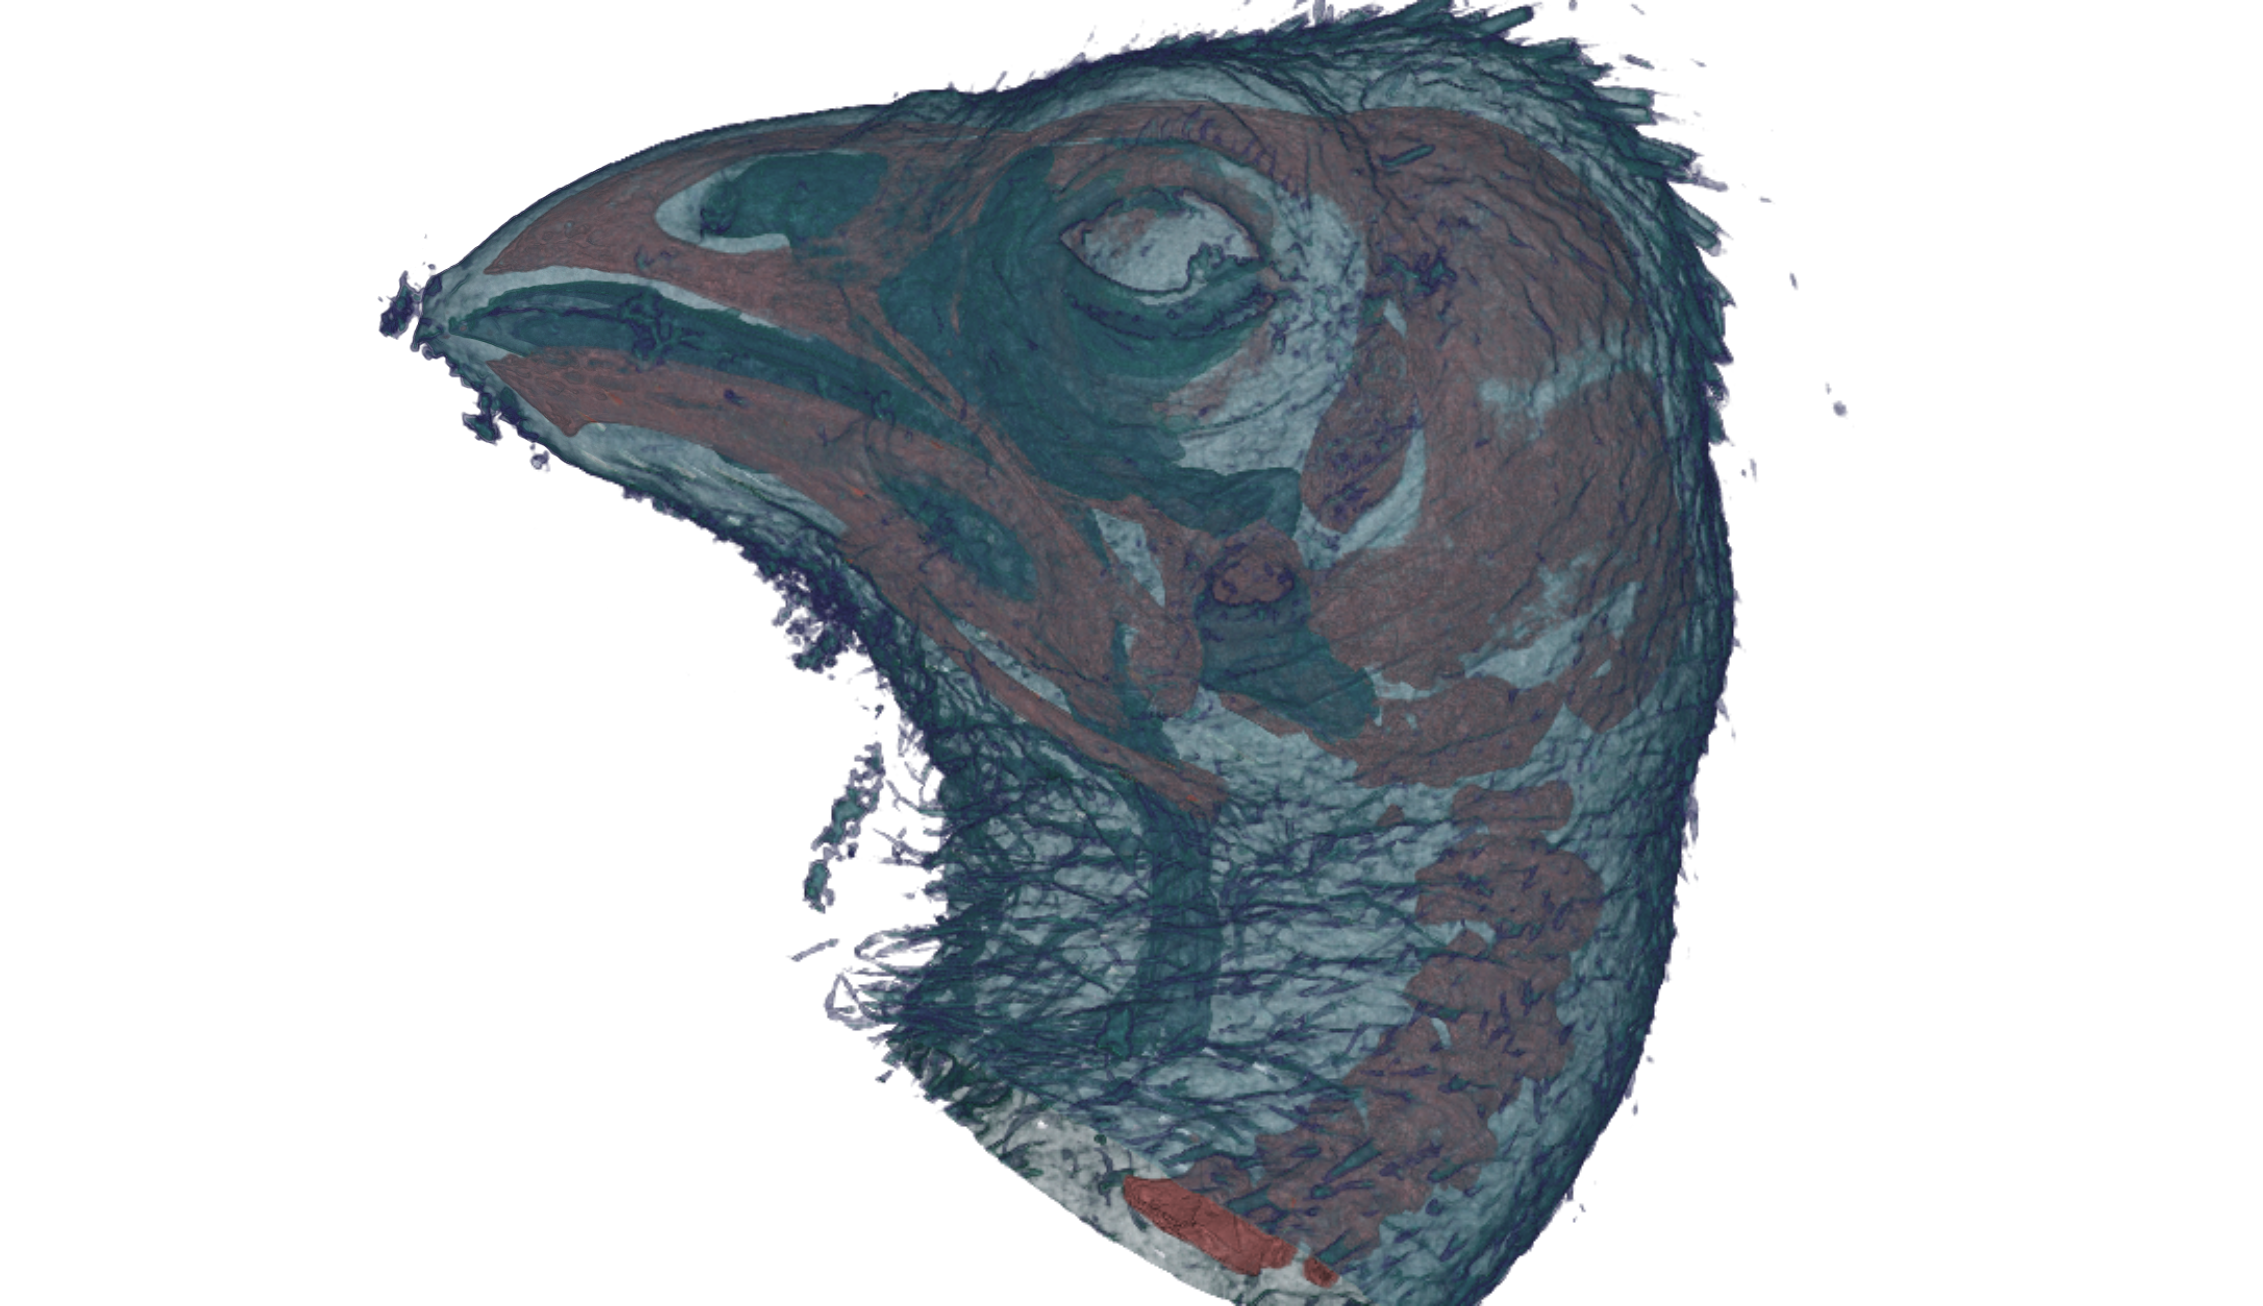
\includegraphics[width=1\textheight]{../../Grafiken/results/picture_quality/hoatzin/MDC_img-0-96_ray-1-5.png}
		\caption{Volumen Hoatzin mit \emph{MDC} Raycast berechnet.}
		\label{fig::res::hoa_mdc}
	\end{figure}
\end{landscape}

\begin{landscape}
	\begin{figure}
		\centering
		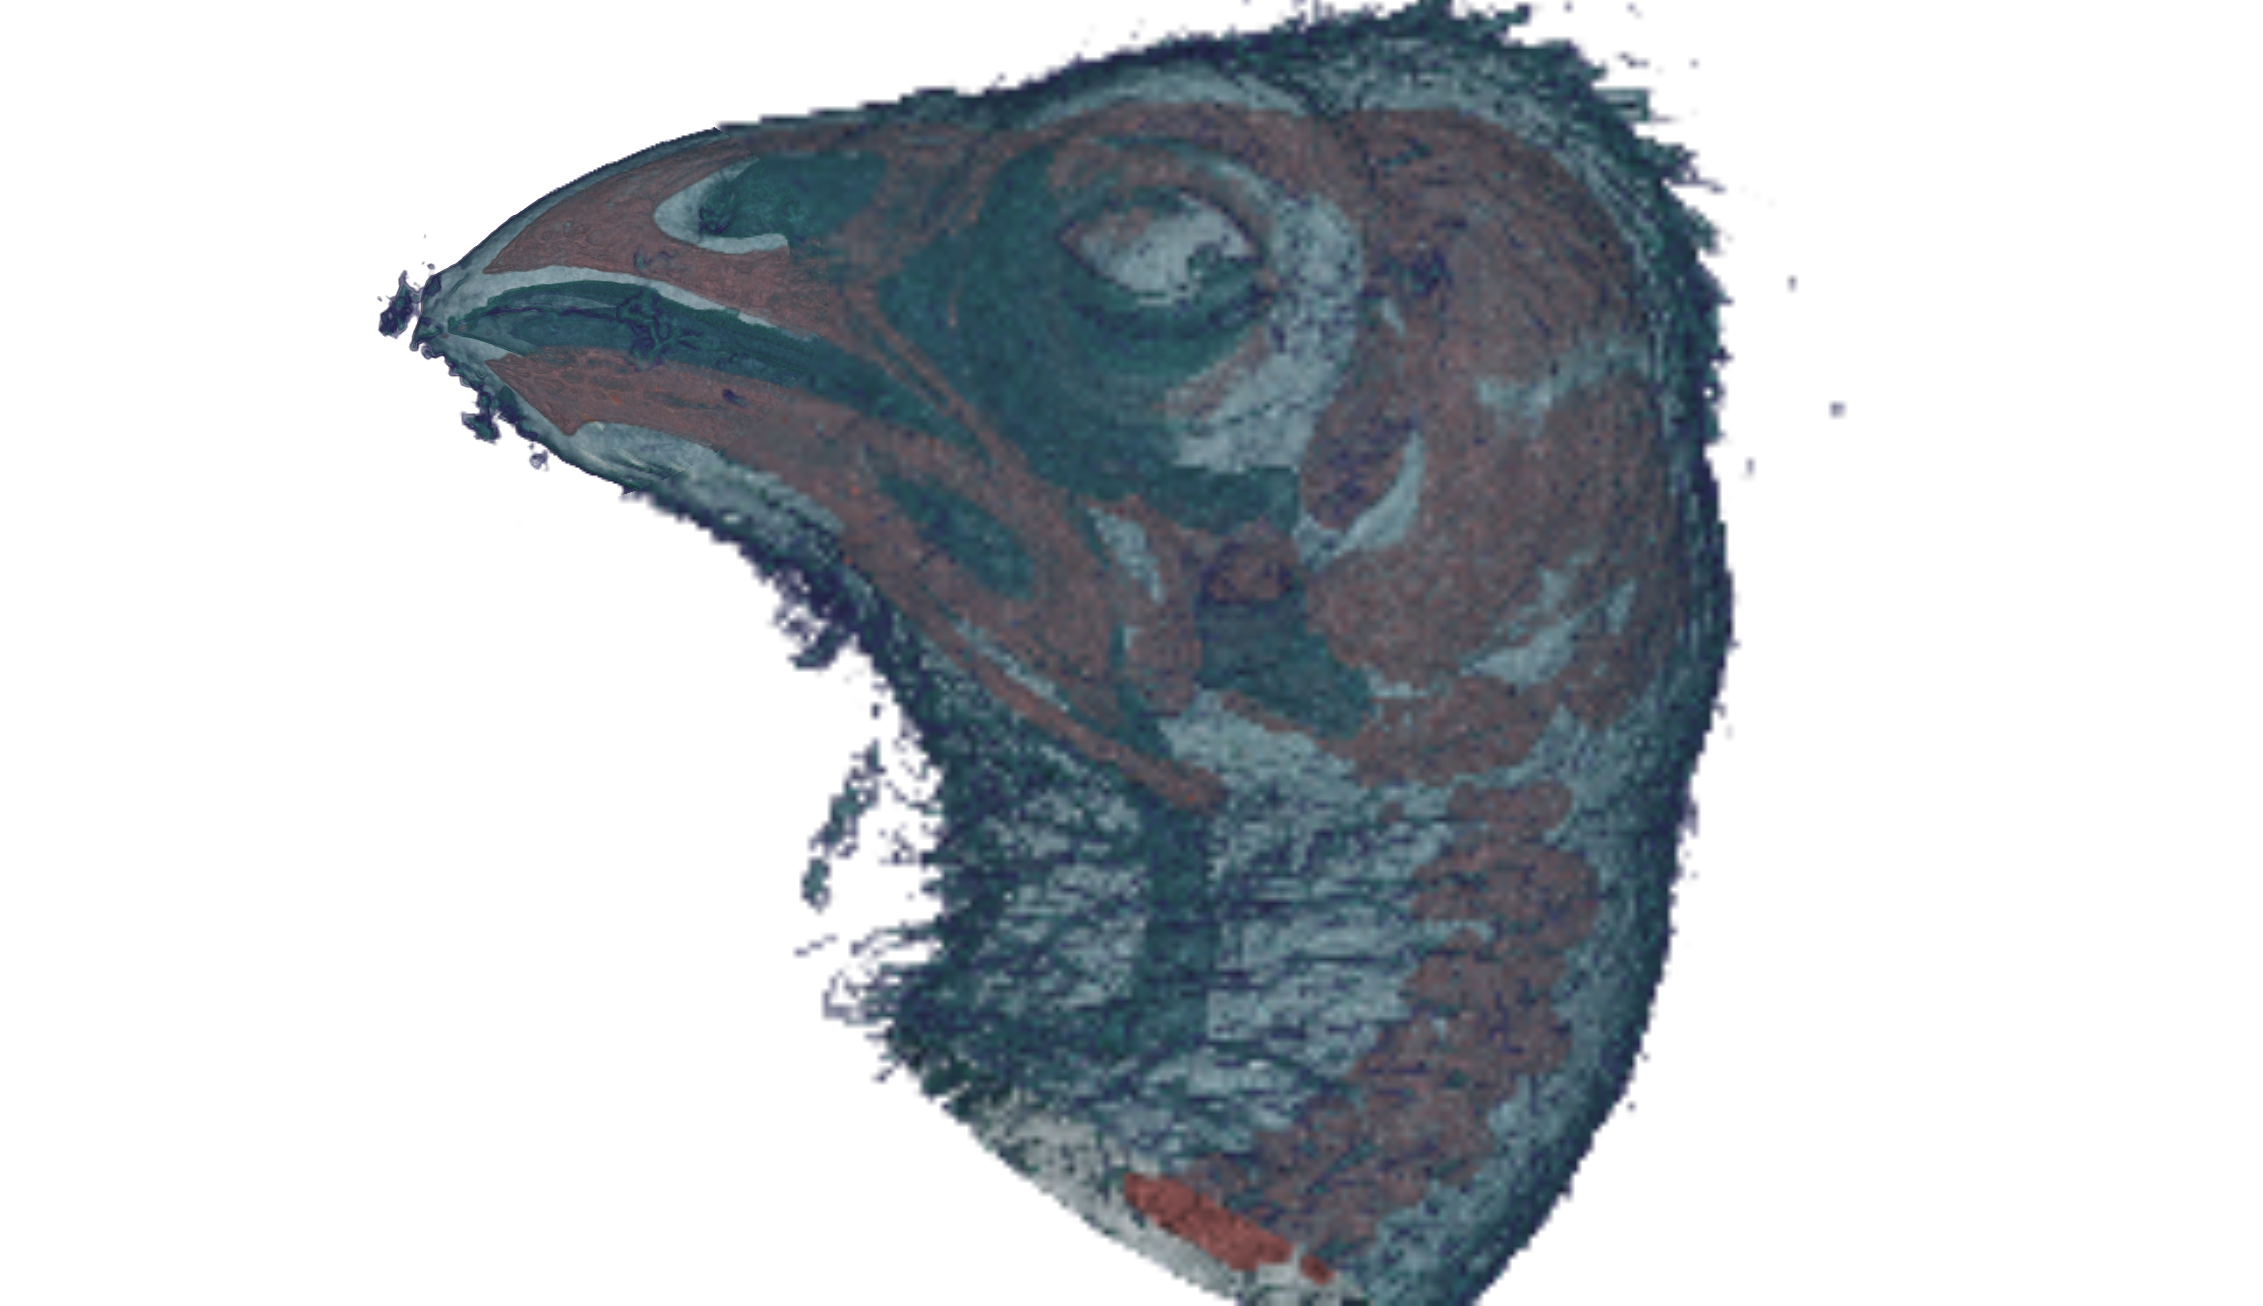
\includegraphics[width=1\textheight]{../../Grafiken/results/picture_quality/hoatzin/DDC_img-1_ray-1-5.png}
		\caption{Volumen Hoatzin mit \emph{DDC} Raycast berechnet.}
		\label{fig::res::hoa_ddc}
	\end{figure}
\end{landscape}
\fi

\subsection{Performanz}





\todo{Messbare Ergebnisse der Arbeit. (Performanzmessungen..).}

\section*{Diskussion}\label{sec::disc}
\todo{Diskussion und Bedeutung der Ergebnisse.}